\documentclass[british]{article}
\usepackage[T1]{fontenc}
\usepackage[latin9]{inputenc}
\usepackage{geometry}
\geometry{verbose,tmargin=3cm,bmargin=3cm,lmargin=3cm,rmargin=3cm,headheight=1cm,headsep=1cm,footskip=2cm}
\usepackage{fancyhdr}
\pagestyle{fancy}
\setlength{\parskip}{\bigskipamount}
\setlength{\parindent}{0pt}
\usepackage{babel}
\usepackage{units}
\usepackage[squaren]{SIunits}
\usepackage{pdfpages}
\usepackage{amsmath}
\usepackage{amssymb}
\usepackage{graphicx}
%\usepackage{mathtools}
\hyphenpenalty=50
\usepackage[font=small,labelfont=bf,textfont=it]{caption}
\usepackage{esint}
\usepackage[unicode=true,
 bookmarks=true,bookmarksnumbered=true,bookmarksopen=true,bookmarksopenlevel=2,
 breaklinks=false,pdfborder={0 0 0},backref=false,colorlinks=false]
 {hyperref}
\hypersetup{pdftitle={Statistical Physics and Entropy},
 pdfauthor={Josh Wainwright}}
\providecommand{\tabularnewline}{\\}
\makeatletter

\newcommand{\lyxdot}{.}
\renewcommand{\d}{\mathrm{d}} % for integrals
\newcommand{\dx}[2]{\frac{\textrm{d} #1}{\textrm{d} #2}} % for derivatives
\newcommand{\dd}[2]{\frac{\textrm{d}^2 #1}{\textrm{d} #2^2}} % for double derivatives
\newcommand{\pd}[2]{\frac{\partial #1}{\partial #2}} % for partial derivatives
\newcommand{\pdd}[2]{\frac{\partial^2 #1}{\partial #2^2}} % for double partial derivatives
\renewcommand{\u}[1]{\underline{#1}} % for underline's vectors
\newcommand{\sintertext}[1]{\intertext{#1}\\[-0.7cm]}

\makeatother

\begin{document}

\title{Statistical Physics and Entropy}

\date{}

\author{Josh Wainwright}

\maketitle

\tableofcontents

\newpage

\part{Statistical Physics}

\section{The Isothermal Atmosphere}

Consider a column of gas at a uniform temperature, $T$, in equilibrium under gravity. How does the pressure, $p$, vary with height?

The downward force on an element due to gravity is given by $gdM$ and the net upward force from the pressure of the container is given by $pA-(p+\d{p})A=-A\d{p}$. 
\begin{align*}
\Rightarrow-A\d{p} & =g\d{M}
\sintertext{But $\d{M}=\rho A\d{z}$,} 
-A\d{p} & =g\rho A\d{z}\\
\dx{p}{z} & =-g\rho
\end{align*}
Where $\rho$ is the density of the the gas at a height $z$ so that $A\d{z}=$volume of unit element. This is "hydrostatics equilibrium" (for a liquid, $\rho$ does not depend
on $z$ so this can be integrated to get $p=\rho gh$). For molecules of mass $m$, the density is given by $\rho=mn$ where n is the number density (the number of molecules per unit volume).


\subsection{Ideal Gas Law}
For one mole of an ideal gas with pressure $p$ and volume $V$ at temperature $T$, 
\begin{align*}
	pV &= RT
	\sintertext{where $R=8.31 \joulepermolekelvinnp$ (the gas constant)}
	R &= N_{A}k
\end{align*}
where $N_{A}=6.02\times10^{23} \reciprocal\mole$ (Avogadro's constant), and $k=1.38\times10^{-23}$ (Boltzmann's constant). Hence, 
\begin{align*}
pV & =N_{A}kT\\
p & =\frac{N_{A}}{V}kT
\end{align*}
 But $\frac{N_{A}}{V}$ is the number density $n$ so the ideal gas law can be written as, 
\begin{align*}
p & =nkT
\end{align*}


\subsection{The Atmosphere}

Since $\dx{p}{z}=-g\rho=-gmn$, and $p=nkT$, we can write the hydrostatic equilibrium as, 
\begin{align*}
\dx{p}{z} & =-\left(\frac{mg}{kT}\right)p
\sintertext{If $T$ is constant, then this can be evaluated as,}
p &= p_{0}e^{-\frac{mgz}{kT}}
\end{align*}
 So the pressure decreases exponentially with height. It is also colder the higher up you go, so the atmosphere is not strictly isothermal, but this can be averaged to get a constant temperature that still
is accurate. Given $p=nkT$, so that $p$ is directly proportional to $n$, this can be written in terms of the number density, 
\begin{align*}
n & =n_{0}e^{-\frac{mgz}{kT}}
\end{align*}
 At any given instant, most molecules are in the region of high density $\left(\text{where }z<\frac{kt}{mg}\right)$. On average, any given molecule must spend most of its time in this region. So, the number
density, $n$, must be a measure of the probability distribution for finding a molecule at different positions in the column.

For gas molecules of mass $m$ in equilibrium at temperature $T$ in a gravitational field, the number density is, 
\begin{align*}
n(z) & =n_{0}e^{-\frac{mgz}{kT}}
\sintertext{Probability density $P(z)$ is proportional to the number density $n(z)$,}
P(z) & =P_{0}e^{-\frac{mgz}{kT}}
\end{align*}
From this, $P(zP)\d{z}$ is the probability of a molecule having a height $z$ to $z+\d{z}$. The constant $P_{0}$ can be determined from the normalisation condition, 
\begin{align*}
\int_{0}^{\infty}P(z)\d{z}=1
\end{align*}


\subsection{The Boltzmann Distribution}

This distribution, $P(z)$ is an example of the Boltzmann Distribution,
\begin{align*}
\text{Probability of having energy }E & \propto e^{-\frac{E}{kT}}
\end{align*}
This can be modified to a probability density if $E$ is continuous. Or more generally, 
\begin{align*}
\text{Probability of having energy }E & \propto(\text{number of ways of having energy }E)\times e^{-\frac{E}{kT}}
\end{align*}


\section{Molecular Velocity and Speed Distributions}
\subsection{Distributions}
\subsubsection{Discrete Distributions}

These are distributions that contain a definite number of possible outcomes, e.g.\ coin tossing, throwing die, etc. If events are discrete and independent, 
\begin{align*}
p_{i} & =\frac{\text{Number of successes}}{\text{Number of trial}}=\frac{N_{i}}{N}
\end{align*}
Let $N\rightarrow\infty$ for this to be a definition of $p_{i}$. The probability $p_{i}$ is a number between 0 and 1, for mutually exclusive events, 
\begin{align*}
\sum_{i}N_{i} & =N\qquad\Rightarrow\sum_{i}p_{i}=1
\end{align*}
so that it is certain that one of the possible outcomes will happen.


\subsubsection{Continuous Distributions}

These are distributions that can take any value, e.g.\ heights of people, positions or velocities of gas molecules etc. For a continuous variable, $x$, draw a histogram of the number of results between
$x$ and $x+\Delta x$. The bar height is proportional to the size of the interval, $\Delta x$, but the height decreases as $\Delta x\rightarrow0$. To overcome this, plot the number density, $n(x)$, 
\begin{align*}
n(x) & =\frac{\text{Number in }x\text{ to }(x+\Delta x)}{\Delta x}
\end{align*}
As $\Delta x\rightarrow0$, the histogram for $n(x)$ approaches a smooth curve (assuming the total number of results $N\rightarrow\infty$)
\begin{align*}
\text{Number in }x\text{ to }x+\d{x} & =n(x)\d{x}\\
\text{Area under the curve} & =\int n(x)\d{x}
\end{align*}
such that the range of integration includes all possible values of $x$.

Define the probability density to be, 
\begin{align*}
P(x) & =\frac{n(x)}{N}
\end{align*}
where $N\rightarrow\infty$. So for a finite region $a$ to $b$, the probability is given by 
\begin{align*}
P(x)_{[a,b]} & =\int_{a}^{b}P(x)\d{x}
\end{align*}


\subsection{Velocity Distribution}

Molecular kinetic energy is given by, 
\begin{align*}
\frac{1}{2}mv^{2} & =\frac{1}{2}m(v_{x}^{2}+v_{y}^{2}+v_{z}^{2})
\end{align*}
Consider each component separately. $P(v_{x})\d{v_{x}}$ is the probability of a molecule having $v_{x}$ to $v_{x}+\d{v_{x}}$. The contribution from $v_{x}$ to the kinetic energy is $\frac{1}{2}mv_{x}^{2}$. Hence the Boltzmann theorem becomes 
\begin{align*}
P(v_{x}) & \propto e^{-\frac{mv_{x}^{2}}{2kT}}\\
P(v_{x}) & =P_{0}e^{-\frac{mv_{x}^{2}}{2kT}}
\end{align*}
This is a Gaussian distribution with a quadratic dependence on the velocity, where $P_{0}$ is a normalisation constant.

This graph is symmetrical between $+v_{x}$ and $-v_{x}$ with a peak at $v_{x}=0$ suggesting that this is the most probable velocity.

\subsection{Speed Distribution}

Let $F(v)\d{v}$ be the probability of a molecule having a speed $v$ to $v+\d{v}$. So the velocity vector must lie inside a spherical shell from $v$ to $v+\d{v}$. 
\begin{align*}
F(v)\d{v} & \propto(\underbrace{\text{number of ways of having \ensuremath{v}to \ensuremath{v+\d{v}}}}_{\propto4\pi v^{2}\d{v}})\times e^{-\frac{mv^{2}}{2kT}}\\
F(v) & =4\pi v^{2}F_{0}e^{-\frac{mv^{2}}{2k}}
\end{align*}


\subsection{Normalised Probability Distributions}

\begin{center}
\begin{tabular}{c|c}
\textbf{Velocity Distribution}  & \textbf{Maxwell-Boltzmann Speed Distribution}\tabularnewline
\hline \hline
${\displaystyle {P(v_{x})=\sqrt{\frac{m}{2\pi kT}}e^{-\frac{mv_{x}^{2}}{2kT}}}}$  & ${\displaystyle {F(v)=\left(\frac{m}{2\pi kT}\right)^{\frac{3}{2}}4\pi v^{2}e^{-\frac{mv^{2}}{2kT}}}}$\tabularnewline
\parbox[c]{23em}{%
\includegraphics{"Statistical Physics and Entropy/Gaussian_speeds".pdf}} & \parbox[c]{23em}{\includegraphics{"Statistical Physics and Entropy/Maxwell_Boltzmann_speeds".pdf}
}\tabularnewline
${\displaystyle {\int_{-\infty}^{+\infty}P(v_{x})\d{v_{x}}=P_{0}\int_{-\infty}^{+\infty}e^{-\frac{mv_{x}^{2}}{2kT}}\d{v_{x}}=1}}$  & ${\displaystyle {\int_{0}^{\infty}F(v)\d{v}=4\pi F_{0}\int_{0}^{\infty}v^{2}e^{-\frac{mv^{2}}{2kT}}\d{v}=1}}$\tabularnewline
\end{tabular}
\par\end{center}


\section{Averages}


\subsection{Discrete Distributions}

Suppose the variable $x$ takes discrete values $x_{i}$ with probabilities $p_{i}$. The average, or mean, of $x$ is given by, 
\begin{align*}
\overline{x} & =\langle x\rangle=\sum_{i}\frac{N_{i}x_{i}}{N}=\sum_{i}x_{i}p_{i}\\
\overline{x^{2}} & =\sum_{i}x_{i}^{2}p_{i}\\
x_{\text{RMS}} & =\sqrt{\overline{x^{2}}}\\
\overline{\Delta x^{2}} & =\sum_{i}\left(x_{i}-\overline{x}\right)^{2}p_{i}=\overline{x^{2}}-{\overline{x}}^{2}=\sigma^{2}
\end{align*}
where $x_{\text{RMS}}$ is the root mean squared speed, $\overline{\Delta x^{2}}$ is the mean-square deviation, or variance and $\sigma^{2}$ is the standard deviation.


\subsection{Continuous Distributions}

Suppose now that $x$ is a continuous variable with normalised probability density $P(x)$, 
\begin{align*}
\overline{x} & =\int xP(x)\d{x}\\
\overline{x^{2}} & =\int x^{2}P(x)\d{x}
\end{align*}
where the range of integration includes all possible values of $x$.


\subsection{Kinetic Theory}

\begin{alignat*}{2}
\overline{v_{x}} & =\int_{-\infty}^{+\infty}v_{x}P(v_{x})\d{v_{x}}=0 & \qquad & \text{Symmetrical distribution}\\
\overline{v} & =\int_{0}^{\infty}vF(v)\d{v}=\sqrt{\frac{8kT}{\pi m}} &  & \text{Mean speed}\\
\overline{v_{x}^{2}} & =\int_{-\infty}^{+\infty}v_{x}^{2}P(v_{x})\d{v_{x}}=\frac{kT}{m} &  & \text{Mean-square velocity}\\
\overline{v^{2}} & =\int_{0}^{\infty}v^{2}F(v)\d{v}=\frac{3kT}{m} &  & \text{Mean-square speed}\\
\end{alignat*}



\subsection{Equipartition of Energy}

\begin{align*}
\overline{v_{x}^{2}} & =\frac{kT}{m}\\
\Rightarrow\frac{1}{2}m\overline{v_{x}^{2}} & =\frac{1}{2}kT\\
\frac{1}{2}m\overline{v^{2}} & =\frac{1}{2}m\overline{v_{x}^{2}}+\frac{1}{2}m\overline{v_{y}^{2}}+\frac{1}{2}m\overline{v_{z}^{2}}
\end{align*}
This is the average kinetic energy given the velocity components of a particle. The principle of equipartition says that the average energy equals $\frac{1}{2}kT$ per degree of freedom, i.e.\ $\frac{1}{2}kT$ for each independent quadratic term in internal energy.

\section{Molecular Collisions}

\subsection{Molecular Collisions with a Wall}
Joule's six stream approximations says that at any one time, there are likely to be $\frac{n}{6}$ molecules travelling towards each face a of unit cube, with speed $v$. This means that the collision rate per unit area will be $\frac{nv}{6}$. When the velocity distribution is taken into account, the more accurate value of $\frac{n\overline{v}}{4}$ was calculated, where $n$ is the number density of the molecules inside the cube.

The Lennard-Jones 6-12 potential, given by
\begin{align*}
	V(r) &= 4\varepsilon \left[ \left(\frac{D}{r}\right)^{12}-\left(\frac{D}{r}\right)^6 \right]
\end{align*}
gives a strong repulsion for very close proximity's, and a weak attraction when the molecules are further away. This is often simplified to the hard-sphere model because of the strong repulsion which leads to the van der Waals radius $R$ which is half the distance between the centres of two neighbouring molecules.

\subsection{Intermolecular Collisions}
Molecules collide if the impact parameter, $b<D$. A stationary molecule presents a target area of  $\pi D^2$, thus giving the scattering cross section $\sigma = \pi D^2$.

Consider a slice of gas of thickness $\d{x}$ and area $A$. The volume of such a slice, then, is given by 
\begin{align*}
	V &= A\d{x}
\end{align*}
Each slice contains $nA\d{x}$ molecules and each molecule in the slice presents a target area of $\sigma$ to any incident molecule on this slice. So the effective scattering area is
\begin{align*}
	A_{\text{scatter}} &= nA\d{x} \\
	\text{Scattering probability} &= \frac{\text{Target area}}{\text{Total area}} \\
	\text{Probability of scattering in }\d{x} &= \frac{nA\d{x}\sigma}{A} = n\sigma\d{x}
\end{align*}

\subsection{Attenuation of a Molecular Beam}
If $N$ molecules are incident on a slice of gas of width $\d{x}$, the the number of molecules leaving the slice with be decreased to $N+\d{N}$ where $\d{N}$ is negative and $\d{N}=-Nn\sigma\d{x}$. For a beam of $N$ molecules, 
\begin{align*}
	\dx{N}{x} &= -n\sigma N \\
	N &= N_0 e^{-n\sigma x}
\end{align*}

\subsection{Mean-Free Path}
The probability  of travelling a distance $x$ without scattering is
\begin{align*}
	P_0 = \frac{N}{N_0} &= e^{-n\sigma x} = e^{-\frac{x}{l}}
\sintertext{So the mean free path is given by}
	l &= \frac{1}{n\sigma}
\sintertext{which for gas molecules becomes}
	l &= \frac{1}{\sqrt{2}n\sigma}
\end{align*}
In air at STP, the mean free path, $l\approx 1 \micro\metre$.

\subsubsection{Distribution of Free Paths}
$P(x)\d{x} =$ Probability of next collision in $x$ to $x + \d{x}$, where $x$ is the free path of a molecule.

Probability of next collision in $x$ to $x + \d{x}$ is equal to the probability of reaching $x$ without scattering times the probability of a collision in $\d{x}$.
\begin{align*}
	P(x)\d{x} &= e^{-n\sigma x} n\sigma x \\
	&= e^{-\frac{x}{l}} \frac{x}{l} \\
	P(x) &= e^{-\frac{x}{l}} \\
	\overline{x} &= \int_0^x xP(x)\d{x} = l
\end{align*}
So the free path is the average distance to the next collision which is equal to the average distance between collisions.

\subsection{Poisson Distribution}
Collisions obey Poisson statistics. Imagine splitting the distance $x$ into many small elements of width $\delta x$. The average number of collisions in $x$ is
\begin{align*}
	\mu &= \left(\frac{x}{\delta x}\right)\times\left(\frac{\delta x}{l}\right) = \frac{x}{l} 
\end{align*}
where $\left(\frac{x}{\delta x}\right)$ is the number of elements and $\left(\frac{\delta x}{l}\right)$ is the probability of a collision in an element $\delta x$. It can be shown that the probability of $r$ collisions in $x$ is 
\begin{align*}
	P_r &= \frac{\mu^r}{r!}e^{-\mu} \qquad \text{Poisson Distribution}
\end{align*}
This also applies to counting particles in nuclear and particle physics ($\mu$ is the average number of counts in the time interval $\Delta t$).
\begin{align*}
	\Rightarrow P_0 &= e^{\mu}
\end{align*}

\subsection{The Crookes Radiometer}
The Crookes Radiometer is a device that spins when a bright light is shined on it. The immediate assumption is that it is radiation pressure that drives the vanes around, but the there are several reasons why this cannot be the case.
\begin{itemize}
	\item Radiation pressure is far too small an effect.
	\item The vanes would spin in the other direction as the black sides are seen to be trailing, not leading.
	\item The bulb contains a low pressure gas, but the vanes do not rotate under a high vacuum or if the density of the gas is any higher.
\end{itemize} 
The vanes are coloured differently. One side of each vane is silvered while the other is black. The black side gets hotter than the silver surface, so adsorption and desorption of molecules by vanes becomes important.

The low pressure inside the bulb means that the free path is greater than the size of the vanes. This means that the adsorbed molecules have approximately the same temperature as the glass bulb. Molecules then desorbed from the black surface are hotter so leave with a higher speed and so exert a higher pressure. This causes the vanes to spin, silver side leading.

\subsection{Effusion}


\begin{minipage}[t]{1\columnwidth}%
\noindent \begin{center}
\includegraphics{"Statistical Physics and Entropy/effusion"}
\par\end{center}%
\end{minipage}

Molecules escape from the chamber by random collisions with a tiny pinhole. The size of the pinhole must be slightly smaller than the molecular mean free path so that the molecules do not simply move by diffusion. Under these circumstances, there is no fluid flow since the hole does not affect the molecular velocities. The rate of effusion is given by $\frac{1}{4}n\overline{v}\delta A$ where $\delta A$ is the area of the pinhole.

The atomic and molecular beams that are produced are used in spectroscopy and in molecular beam epitaxy e.g.\ Ammonium sulphate is $\text{GaAl}_x\text{As}_{1-x}$.

\section{Diffusion}

Diffusion is the flux $J_x$ from high to low concentration due to the random motion of particles. It is defined by Fick's law,
\begin{align*}
	J_x &= -D\pd{n}{x}
\end{align*}
where $D$ is the diffusion coefficient, the flux $J_x$ is measured in number per unit area per second and $\pd{n}{x}$ is the number density gradient which normally depends on time as well as the three spacial dimensions. The flux can be calculated from the six-stream approximation,
\begin{align*}
	J_1 = \frac{1}{6}\left( n-l\pd{n}{x} \right) \overline{v} \quad &\text{and}\quad J_2 \frac{1}{6} \left( n+ l\pd{n}{x} \right) \overline{v} \\
	\Rightarrow J_x = J_1 - J_2 &= -\frac{1}{3}\overline{v}l\pd{n}{x} = -D\pd{n}{x}
\end{align*}
This means that the diffusion coefficient is given by
\begin{align*}
	D &= \frac{1}{3}\overline{v}l
\sintertext{If rigorous theory is used, the value of the coefficient is}
	D &= \frac{1}{4}\overline{v^2}\tau
\sintertext{where $\tau$ is the mean free time, or the average time between collisions,}
	\tau &= \frac{l}{\overline{v}}
\end{align*}

\subsection{Mobility}
Suppose particles undergo random collisions in the presence of an applied force, $F$. The applied force produces a constant acceleration $a=\frac{F}{m}$. Suppose the velocity immediately after the last collision at $t=0$ is $u$. So the average over many collisions is 
\begin{align*}
	\langle v \rangle &= \langle u \rangle + \frac{F\langle t \rangle}{m} \\
	&= \langle u \rangle + \frac{F\tau}{m}
\end{align*} 
If we assume the collisions randomise the initial velocity $u \Rightarrow \langle u \rangle =0$, and so the average velocity $\langle v \rangle = \frac{F\tau}{m}$. The applied force $F$ produces a steady drift velocity $V_{\text{drift}}$.
\begin{align*}
	\text{Drift velocity} \quad v_{\text{drift}} &=\frac{F\tau}{m} = \mu F \\
	\text{Mobility} \quad \mu &=\frac{\tau}{m}
\end{align*}

\subsection{Transport Coefficients}

\[
 \begin{array}{r c r l c r l}
  \text{Mobility } \mu :& \quad & v_{\text{drift}} &= \mu F & \quad & \mu &= \displaystyle{\frac{\tau}{m}}\\ \\
  \text{Diffusion Coefficient } D  :&& \text{Flux } J_x &= -D\displaystyle{\pd{n}{x}} && D &=\displaystyle{\frac{1}{3}}\overline{v}l \\ \\
  \text{Viscocity } \eta :&& \text{Shear force} &= -\eta A\displaystyle{\pd{V_x}{y}} && \eta &= \displaystyle{\frac{1}{3}\rho \overline{v}l} \\ \\
  \text{Thermal Conducitivity } K :&& \text{Heat flow } \dot{Q}_x &= \displaystyle{-KA\pd{T}{x}} && K&= \displaystyle{\frac{1}{3}C_V\overline{v}l} \\ \\
  \text{Electrical Conducitivity } \sigma :&& \text{Current density } j &= \sigma E && \sigma &= \displaystyle{\frac{ne^2\tau}{m}} \\ \\
 \end{array}
\]

\subsection{Einstein Relation}
The diffusion coefficient is given by
\begin{align*}
	D &= \frac{1}{3}\overline{v^2}\tau = \frac{1}{3}\left( \frac{3kT}{m} \right) \tau = \left(\frac{\tau}{m}\right)kT
\sintertext{Since the mobility is given by $\mu=\frac{tau}{m}$}
	D &= \mu KT
\end{align*}
This is the Einstein Relation. When this is applied to spherical particles or radius $r$ in a medium of viscosity $\eta$, this leads to Stokes Law,
\begin{align*}
	F &= 6\pi \eta r v
\end{align*}
The applied force $F$ produces a steady drift velocity $v_{\text{drift}}$ given by
\begin{align*}
	v_{\text{drift}} &= \frac{F}{6\pi\eta r} = \mu F
\sintertext{Since the mobility is given by}
	\mu &= \frac{1}{6\pi \eta r}
\sintertext{the diffusion coefficient can be written as}
	D &= \mu kT  = \frac{kT}{6\pi \eta r}
\end{align*}
So the diffusion coefficient is inversely proportional to the radius, a large radius means a small amount of diffusion.

\subsection{Diffusion Equation}
The equation of continuity can be written as 
\begin{align*}
	\pd{n}{t} + \pd{J_x}{x} &= 0
\sintertext{So the diffusion equation is}
	\pd{n}{t} &= D\pdd{n}{x} \\
	n(x,t) &= \frac{N_0}{\sqrt{4\pi Dt}}e^{-\frac{x^2}{4Dt}}
\sintertext{This is a Gaussian relation, where $\sigma^2 = 2Dt$}
	\overline{x^2} = 2Dt &\Rightarrow x_{\text{RMS}}=\sqrt{2Dt} 
\end{align*}
This means that the distance diffused is proportional to $\sqrt{t}$. This is characteristic of diffusion which in three dimensions can be written as 
\begin{align*}
	\overline{R^2}=\overline{x^2}+\overline{y^2}+\overline{z^2}=6Dt
\end{align*}

\section{Brownian Motion}
\subsection{Random Walk}
A random walk in Brownian motion is the movement of a particle due to random applied force. Consider taking $N$ steps of length $a$ in random directions
\begin{align*}
	R &= \sum_i a_i \\
	\overline{R} &= \sum_i \overline{a}_i =0
\end{align*}
The average displacement is zero because the particle is equally likely to step left or right, up or down etc. Hence, find the mean square displacement instead.
\begin{align*}
	R^2 &= R\cdot R = (a_1 + a_2 + \dots a_N)\cdot (a_1 + a_2 + \dots a_N) \\
	&= a_1^2 + a_2^2 + \dots + a_N^2 + (a_1\cdot a_2 + a_1\cdot a_3 + \dots) \\
	&= Na^2 + \sum_{i\neq j} a_i \cdot a_j \\
	\Rightarrow \overline{R^2} &= Na^2 + \sum_{i\neq j}\overline{a_i \cdot a_j}
\sintertext{But $\overline{a_i \cdot a_j}= a^2 \overline{\cos(\theta_i - \theta_j)}=0$}
	\Rightarrow \overline{R^2} &= Na^2
\end{align*}
For $N$ steps of length $a$ in random directions,
\begin{align*}
	\langle R\rangle &= 0 \\
	\langle R^2\rangle &= Na^2
\end{align*}
If the steps occur at a rate of $k_0$, then $N=k_0t$
\begin{align*}
	\Rightarrow \langle R^ \rangle &= k_0a^2t \qquad \text{In one dimension} \\
\sintertext{Hence}
	D &= \frac{k_0 a^2}{2}
\sintertext{In three dimensions, this becomes}
	\langle R^2 \rangle &= 6Dt \\
	D &= \frac{k_0a^2}{6}
\end{align*}
The distribution that describes the motion of particles under diffusion conditions is the Gaussian. For particles undergoing random walks, it is described instead by a Binomial Distribution. This is an unbiased distribution with and average $\langle R \rangle =0$. 

\subsection{Binomial Distribution}
\subsubsection{Binomial Expansion}

The binomial theorem is 
\begin{align*}
	(p+q)^N &= \sum_{r=0}^{N} {}^N C_rp^r q^{N-r}
\sintertext{where ${}^N C_r$ is the binomial coefficient,}
	{}^N C_r &= \frac{N!}{(N-r)!r!} = \frac{N(N-1)(N-2) \ldots (N-r+1)}{r!}
\end{align*}
The binomial coefficient gives the number of ways of choosing $r$ objects out of $N$ possibilities, so is the number of combinations available. $r!$ is the number of ways of ordering $r$ objects, so is the number of permutations.

\subsubsection{Binomial Distribution}
Suppose
\begin{align*}
	p &= \text{Probability of success in a single trial and} \\
	q &= \text{Probability of failure in a single trial.}
\end{align*}
Since success and failure are mutually exclusive events, $p+q=1$ and so $(p+q)^N=1$. Therefore
\begin{align*}
	\Rightarrow \sum_{r=0}^N {}^N C_r p^rq^{N-r} &= 1
\end{align*}
So now $N\choose r$ is number of ways of obtaining $r$ successes in $N$ trails, and $p^rq^{N-r}$ is the probability of any particular one of these ways occurring. Hence, the probability, $P(r,N)$, of $r$ successes in $N$ trials is given by
\begin{align*}
	P(r,N) &= {}^N C_r p^r q^{N-r}
\end{align*}
This is the binomial distribution. 

\subsubsection{Mean and Variance}
Let $\mu$ be the mean number of successes in $N$ trials and $\sigma^2$ be the variance in $r$. So, $\mu = \overline{r}$ and $\sigma^2 = \overline{r^2} - \overline{r}^2$. It can be shown that 
\begin{align*}
	\mu &= Np \qquad \text{and} \\
	\sigma^2 &= Npq
\end{align*}
When $p=\frac{1}{2},\; \mu=Np=\frac{N}{2}$, also, $\sigma^2=Npq=\frac{N}{4}$, so $\sigma=\frac{\sqrt{N}}{2}$. Note that $\frac{\sigma}{\mu} = \frac{1}{\sqrt{N}}$.

\subsubsection{Poisson and Gaussian Distributions}
\begin{itemize}
	\item In the limit $N\rightarrow \infty$, for fixed $\mu=Np$,
		\begin{align*}
			P(r,N) \rightarrow P_r &= \frac{\mu^r}{r!}e^{-\mu}
		\end{align*}
	This is the Poisson distribution.
	\item In the limit $N\rightarrow \infty$, for fixed $\sigma^2=Npq$,
		\[
			P(r,N) \rightarrow p(x)\d{x} = \frac{1}{\sqrt{2\pi\sigma^2}}e^{-\frac{(x-\mu)^2}{2\sigma^2}}\d{x}
		\]
	This is the Gaussian or Normal distribution.
\end{itemize}
\u{Ex}

For particles in a box, at any instant, the number of molecules on the LHS and RHS may not be equal. Suppose the number of particles in the right side is $r$, so the number in the left side is $N-r$. Since the side of the box are the same size, the probability of finding a particular particle in either side is equal, $\frac{1}{2}$.

So the probability of $r$ molecules on the right is given by,
\begin{align*}
	P(r,N) &= {}^NC_r \times \left( \frac{1}{2^N} \right)
\end{align*}
The most probable arrangement has $r=\frac{N}{2}$, this is the equilibrium state for this system. Statistics can be used to understand thermal equilibrium.

\part{Thermal Equilibrium}
\section{Micro-states and Entropy}
Again consider the case of particles in a box confined to one side of the box by a partition. When the partition is removed, the gas expands into the vacuum, so that, at equilibrium, each molecule is equally likely to be on the left as on the right hand side.

The probability of finding all $N$ molecules on one side is $\frac{1}{2^N}$. Even for a small  number of molecules, e.g.\ this is enormously large - $\approx 10^{-30}$. So it can be said that the molecules will never all move spontaneously to on side., thus the expansion of the gas is an irreversible process.

The binomial distribution gives the system that is most likely to be found is with half the molecules on each side of the box at any one time. This is the most probably macro-state.

\subsection{Micro-states and Macro-states}
For a system with $N$ particles, there are $2^N$ ways to share then between the two sides of the box(given the particles are distinguishable, unlike in the quantum case), so there are $2^N$ micro-states. A micro-state is a detailed microscopic specification of the state of a system, e.g.\ positions and velocities or quantum states.

With $N$ different particles, with $r$ on one side, ${}^N C_r$ gives the number of possible micro-states corresponding to this one single macro-state, specified by $r$. A macro-state is the specification of a system using only macroscopic constraints, e.g.\ number $r$ on one side, total energy $E$ and volume $V$ etc. So each macro-state has many accessible micro-states.

\subsubsection{Probability of a Micro-state}
A single micro-state represents 1 out of a total $2^N$ separate possibilities. The Principle of Equal A Priori Probabilities says that for an isolated system, all accessible micro-states are equally probable. This is a fundamental assumption of statistical mechanics. So each micro-state has a probability of $\frac{1}{2^N}$ of occurring.

\subsubsection{Probability of a Macro-state}
One macro-state has ${}^NC_r$ accessible micro-states, so the probability of a macro-state $r$ is
\begin{align*}
	P(r,N) &= {}^N C_r \left(\frac{1}{2^N} \right)
\end{align*}
where $\frac{1}{2^N}$ is the probability of a micro-state. The probability of a macro-state is proportional to the number of accessible micro-states, $\Omega$, where $\Omega$ is the statistical weight of the macro-state. For an isolated system, $\Omega$ is a maximum at thermal equilibrium.

\subsection{Boltzmann Entropy}
For a composite system composed of system $A$ and system $B$, the number of micro-states for $A+B$ is given by
\begin{align*}
	\Omega &= \Omega_A\Omega_B \\
	\Rightarrow \ln\Omega &= \ln\Omega_A+\ln\Omega_B
\end{align*}
The Boltzmann entropy is defined as 
\begin{align*}
	S &= k\ln\Omega
\sintertext{So}
	S &= S_A+S_B
\end{align*}

\subsubsection{Counting Micro-states}
If a box of volume $V$ is divided into many small cells of volume $\delta V$, then a particle in the box may be found in any of the separate cells. Each particle has $\frac{V}{\delta V}$ accessible micro-states. This means that there are $\Omega$ different micro-states for $N$ particles in the box where 
\begin{align*}
	\Omega = \left(\frac{V}{\delta V}\right)^N
\end{align*}
For a large volume, the number of micro-states, $\Omega$, is very large and so $S$, the entropy, is large. 
\begin{align*}
	S &= k\ln\Omega = Nk\ln\left(\frac{V}{\delta V}\right)
\end{align*}
But the size of $\delta V$ is arbitrary. Classical physics has no unique way to count micro-states whereas for a quantum system, quantum states are quantised and so can be counted.

\subsection{Entropy and Disorder}
For the particles in a box, when the particles are all on one side, the system is ordered, so there is a small number of states and so a small entropy, and when the particles spread out, the number of possible states increases and so does the degree of entropy associated with the system.
\begin{align*}
	\Omega_1 = \left(\frac{V}{\delta V}\right)^N &\qquad \Omega_2 = \left(\frac{2\times V}{\delta V}\right)^N
\end{align*}
The increase in entropy can be defined
\begin{align*}
	\Delta S &= k\ln\left(\frac{\Omega_2}{\Omega_1} \right) = Nk\ln2
\end{align*}
Now the increase in entropy $\Delta S$ does not depend on the choice of $\delta V$

\section{Temperature and the Boltzmann Distribution}
\subsubsection{Thermally Isolated System}
The probability of a particular micro-state is proportional to the number, $\Omega$. At thermal equilibrium, the number of states is at a maximum. The Boltzmann entropy is defined as $S=k\ln\Omega$, so $S$ is a maximum as well,

\subsection{Zeroth Law of Thermodynamics}
The zeroth law of thermodynamics says
\begin{quote}
	"If systems $A$ and $B$ are in equilibrium and systems $B$ and $C$ are in equilibrium, then systems $A$ and $C$ are also in equilibrium."
\end{quote}
Suppose $B$ is a thermometer, then $A$ and $C$ must be at the same temperature.

\subsection{Absolute Temperature}
If systems $A$ and $VB$ are in thermal contact (with constant $V_A$ and $V_B$), then $S=S_A+S_B$ is a maximum at thermal equilibrium. When we transfer heat $\delta Q$, $\delta S = \delta S_A + \delta S_B=0$. A change in $\delta Q$ is a change in the internal energy of the system, so $\delta U_A = -\delta Q$ and $\delta U_B = \delta Q$.
\begin{align*}
	\Rightarrow& \delta S = \left( \pd{S_A}{U_A} \right)_{V_A} (-\delta Q) + \left(\pd{S_A}{U_A}\right)\delta Q=0 \\
	\Rightarrow& \left(\pd{S_A}{V_A} \right)_{V_A} = \left(\pd{S_B}{U_B} \right)_{V_B}
\end{align*}
Two systems in equilibrium have the same temperature. Define the thermodynamic temperature $T$ by
\begin{align*}
	\frac{1}{T} &= \left(\pd{S}{U}\right)_V \\
	T &= \left(\pd{U}{S}\right)_V
\end{align*}
The units are then defined by natural phenomena, in this case the Kelvin (absolute) temperature scale is defined to have the triple point of water, $T_t=273.16 \kelvin$ and is identical to the ideal-gas scale.

\subsubsection{Heat Bath} 
For a system in thermal contact with a heat bath, energy is exchanged as heat and $V$ is constant. Consider a system in micro-state $i$ with energy $E$, so the probability of each state is $p_i$. For a system and heat bath in contact, the overall situation is an isolated composite entity. At thermal equilibrium, all accessible micro-states of the composite system are equally probable. When the system is in state $i$, the heat bath has $\Omega(E-E_i)$ micro-states. The probability of finding the system in a single micro-state is 
\begin{align*}
	p_i &\propto \Omega(E-E_i)
\end{align*}
Since the heat bath is much larger than the system, it can be assumed that $E \gg E_i$, so
\begin{align*}
	\ln \Omega(E-E_i) &\approx \ln\Omega(E) - E_i \left(\pd{\ln\Omega}{E}\right)_V \\
	\Rightarrow \ln p_i &= C - E_i\left(\pd{\ln \Omega}{E}\right)_V 
\sintertext{But}
	\frac{1}{T} &= \left(\pd{S}{E}\right)_V = k\left(\pd{\ln \Omega}{E}\right)_V \\
	\Rightarrow \ln p_i & \approx C - \frac{E}{kT} \\
	p_i &= e^{-\frac{E_i}{kT}}
\end{align*}
Using the condition that $\sum_i p_i=1$, this function can be normalised to
\begin{align*}
	p_i &= \frac{e^{-\frac{E_i}{kT}}}{Z}
\sintertext{where $Z$ is the partition function, given by}
	Z &= \sum_i e^{-\frac{E_i}{kT}} 
\end{align*}
this is the sum of the Boltzmann factors. This probability distribution, $p_i$ is called the Boltzmann, Canonical or Standard Distribution.

\subsection{Density of States}
The probability $P_n$ of finding a system with energy $E_n$ is 
\begin{align*}
	P_n &= \frac{g_n e^{-\frac{E_i}{kT}}}{Z}
\sintertext{where}
	Z &= \sum_n g_n e^{-\frac{E_n}{kT}}
\end{align*}
This is the sum over all possible energy levels, $E_n$. $g_n$ is the number of states with energy $E_n$ and corresponds to the quantum mechanical quantity of degeneracy. If $E$ is continuous, then a probability density function can be used,
\begin{align*}
	P(E) &= \frac{g(E) e^{-\frac{E}{kT}}}{Z}
\sintertext{where now}
	Z &= \int g(E) e^{-\frac{E}{kT}} \d{E}
\end{align*}
Here $g(E)$ is the density of states for the system, $g(E)\d{E}$ is the number of states with energy $E$ to $E+\d{E}$ and $P(E)\d{E}$ is the probability that a system has energy $E$ to $E+\d{E}$.

\subsection{Fluctuations}
The internal energy of a system is given by
\begin{align*}
	E &= \overline{E} = \sum_i E_i p_i
\sintertext{and the variance by}
	\overline{\Delta E^2} & = \overline{E^2} - \overline{E}^2 = \sum_i E_i^2 p_i - \left( \sum_i E_i p_i\right)^2
\sintertext{From this, it can be shown that}
	\overline{\Delta E^2} &= kT^2 \left(\pd{U}{T}\right)_V = kT^2 C_V \\
	\Rightarrow \frac{\Delta E_{RMS}}{\overline{E}} &= \frac{\sqrt{kT^2C_V}}{\overline{E}}
\end{align*}
where $C_V$ is the heat capacity of the system at constant volume. For $N$ classical particles
\begin{align*}
	\overline{E} &\approx NkT \\
	\Rightarrow C_V &\approx Nk \\
	\Rightarrow \frac{\Delta E_{RMS}}{\overline{E}} &= \frac{\sqrt{kT^2C_V}}{\overline{E}} \approx \frac{\sqrt{kT^2Nk}}{\overline{NkT}} =\frac{1}{\sqrt{N}}
\end{align*}
\begin{itemize}
	\item For $N\approx 1$, $\Delta E_{RMS} \approx \overline{E}$, this says that a macroscopic system undergoes large fluctuations.
	\item For $N \approx 10^{22}$, $\Delta E_{RMS}\approx 10^{-11}\overline{E}$, this says that macroscopic systems undergo tiny fluctuations.
\end{itemize}

\subsection{Statistical Ensembles}
A statistical ensemble is a collection of many similar systems. A fraction $p_i$ of the systems in the ensemble are in state $i$ so we can assume that the average over the ensemble is the same as the time average for a single system. This is the Ergodic Hypotheses.
\begin{align*}
	p_i &= \frac{e^{-\frac{E_i}{kT}}}{Z}
\end{align*}
This is the Canonical Ensemble. The micro-canonical Ensemble (for an isolated system) then is given by
\begin{align*}
	p_i &= \frac{1}{\Omega}
\end{align*}

\section{Equipartition Theorem}
It has been shown that 
\[
	\frac{1}{2}m\overline{v_x^2} = \frac{1}{2}kT
\]
This is independent of the mass of the mass $m$. Internal energy often contain quadratic terms in the form $\frac{1}{2}Aq^2$ where $q$ is a generalised co-ordinate, velocity or momentum, e.g.\ position, velocity, linear momentum, angle, angular momentum, angular velocity etc. From this we can define a degree of freedom. A degree of freedom is an independent quadratic term in the energy equation. For each degree of freedom
\begin{align*}
	\frac{1}{2}A\overline{q^2} &= \frac{1}{2}A\frac{\displaystyle{\int_{-\infty}^{+\infty} q^2 e^{-\frac{Aq^2}{2kT}}}dq}{\displaystyle{\int_{-\infty}^{+\infty} e^{-\frac{Aq^2}{2kT}}}dq} = \frac{1}{2}kT
\end{align*}
The principle of the equipartition of energy says that 
\[
\text{Average energy, }U = (\text{Number of degrees of freedom})\times \frac{1}{2}kT
\]
So, for example,
\[
	\frac{1}{2}m\overline{v^2} = \frac{1}{2}m\overline{v_x^2} + \frac{1}{2}m\overline{v_y^2} + \frac{1}{2}m\overline{v_z^2} = \frac{3}{2}kT
\]

\subsection{Classical Harmonic Oscillator}
The harmonic oscillator is an oscillating system that has certain defining characteristics. Consider a mass $m$ on a spring of stiffness $K$. The angular frequency is given by
\begin{align*}
	\omega &= \sqrt{\frac{K}{m}}
\sintertext{The energy of the system is}
	E&= E_k+E_p = \frac{p_x^2}{2m}+\frac{1}{2}Kx^2
\sintertext{For this particular system, there are 2 degrees of freedom}
	\Rightarrow \overline{E} &= kT
\end{align*}
Atoms in a solid can vibrate in three dimension, this gives rise to the three normal modes per atom, so three harmonic oscillators per atom. Thus the average thermal energy is $3kT$ per atom,
\[
	U = 3RT \qquad \text{(per mole)}
\]
The heat capacity at constant volume, then is
\[
	C_V = 3R
\]
This is the Dulong-Petite law. This is not a bad approximation for insulators at room temperature, however, at low temperatures, $C_V \ll 3R$, due to quantum mechanical effects.

\subsection{Quantum Harmonic Oscillator}
Solving the time independent Schrodinger equation with the energy used in the classical oscillator, the eigen values for the quantum version can be found. The energy levels are found to be is steps according to
\[
	E_n = \left(n+\frac{1}{2}\right)\hbar\omega
\]
where $\omega$ is the classical angular frequency, and $n$ is the quantum number, $1,2,3\ldots$. This shows that the energy of the oscillator is quantised in steps of $\hbar\omega$. Also, the minimum energy, when $n=0$ is not zero. This non-zero minimum is called the zero point energy and is at an energy of $\frac{\hbar\omega}{2}$, this leads to the Heisenberg uncertainty product between the position and velocity, $\Delta p_x\Delta x \ge \frac{\hbar}{2}$.

\subsection{Einstein Theory (1907)}
The average number of quanta at temperature $T$ is given by
\begin{align*}
	\overline{n} &= \sum_{n=0}^\infty np_n = \frac{1}{Z}\sum_{n=0}^\infty ne^{-\frac{n\hbar\omega}{kT}}
\end{align*}
where
\begin{align*}
	Z &=\sum_{n=0}^\infty e^{-\frac{n\hbar\omega}{kT}} = 1 + e^{-\frac{\hbar\omega}{kT}} + e^{-\frac{2\hbar\omega}{kT}} + \ldots = \frac{1}{1-e^{-\frac{\hbar\omega}{kT}} }\\
	\sum_{n=0}^\infty ne^{-\frac{n\hbar\omega}{kT}} &= \sum_{n=0}^\infty ne^{-nx} = -\pd{}{x}\left(\sum_{n=0}^\infty ne^{-nx} \right) = \frac{e^{-x}}{\left(1-e^{-x}\right)^2}
\end{align*}
where $x=\frac{\hbar\omega}{kT}$.

\subsection{Heat Capacity}
The average energy of a system is given by
\begin{align*}
	U &= \left(\overline{n}+\frac{1}{2}\right)\hbar\omega = \frac{\hbar\omega}{e^{\frac{\hbar\omega}{kT}}-1}+\frac{\hbar\omega}{2}
\end{align*}
At high temperatures, when $kT\gg \hbar\omega$, the equation becomes the same as for the Equipartition theorem, this is the classical limit, $U\approx kT$, and so the heat capacity becomes
\[
C_V = \left(\pd{U}{T}\right)_V = k
\]
At low temperatures, when  $kT\ll \hbar\omega$,
\begin{align*}
	U &\approx \hbar\omega e^{-\frac{\hbar\omega}{kT}}+\frac{\hbar\omega}{2} \\
	\Rightarrow C_V &\approx \frac{(\hbar\omega)^2}{kT^2}e^{-\frac{\hbar\omega}{kT}}
\end{align*}
So the vibrations freeze out when $kT\ll \hbar\omega$. This applies to the heat capacity of solids and the molecular vibrations in gasses (e.g.\ H$_2$).

\subsubsection{Heat Capacity of Solids}
Einstein treated atoms in a solid as independent oscillators all with the same frequency. Using this he derived the Einstein temperature, given by
\[
	\Theta_E = \frac{\hbar\omega}{k}
\]
But in fact, the atoms act as coupled oscillators. Low frequency vibrations are sound waves (with wavelength much greater tan the atomic spacing), the quanta of which are known as \emph{phonons}, instead of photons for electromagnetic waves.

\subsubsection{LC Circuit}
As with the classical harmonic oscillator in the spring-mass system, the same laws govern other harmonic oscillators, such as is found in a LC circuit.
\[
	E +\frac{1}{2}LI^2 + \frac{1}{2}CV^2
\]
where now $\omega =\sqrt{\frac{1}{LC}}$. Both oscillators have 2 degrees of freedom, so the Equipartition theorem can be applied, meaning the average thermal energy is $kT$. Thermal noise fluctuations apply when $kT \gg \hbar\omega$.

\section{Black Body Radiation}

\subsection{Electromagnetic Cavity Modes}
Electromagnetic standing waves inside a conducting box are referred to as cavity modes, where the box represents the cavity resonator. The electromagnetic energy inside the box is given by
\[
	U = \int \left(\frac{1}{2}\varepsilon_0 E^2 + \frac{B^2}{2\mu_0}\right) \d{V}
\]
The first term is the electric energy, or the potential energy of the system, and the second term is the magnetic, or kinetic energy of the system. Each cavity mode behaves like a harmonic oscillator. In quantum field theory, we can apply quantum mechanics to the electromagnetic field, so that $\hat{E_k} \approx \hat{x}$ and $\hat{B_k} \approx \hat{p_x}$.  So now the cavity mode is equivalent to the quantum harmonic oscillator. The energy of each mode is restricted to 
\[
	E = \left(n+\frac{1}{2}\right) h\nu
\]
where there are $n$ photons in the cavity mode.

\subsection{Black Body Spectrum}
The average energy of a mode of frequency $\nu$ at temperature $T$ is
\[
	\overline{E} = \left(\overline{n}+\frac{1}{2}\right) h\nu = \frac{h\nu}{e^{\frac{h\nu}{k_BT}}-1} + \frac{h\nu}{2}
\]
Let $g(\nu)\d{\nu}$ be the number of modes with a frequency between $\nu$ and $\nu+\d{\nu}$. It can be shown that $g(\nu)\propto\nu^2$ because there are $k$ vectors is a spherical shell $4\pi k^2 \d{k}$. Also let $u(\nu)\d{\nu}$ be the energy per unit volume between $\nu$ and $\nu+\d{\nu}$.
\[
	\Rightarrow u(\nu) = \frac{g(\nu)h\nu}{e^{\frac{h\nu}{k_BT}}-1} = \frac{8\pi h}{c^3} \frac{v^3}{e^{\frac{h\nu}{kT}}-1}
\]
This is Plank's Law.

The Equipartition theory predicts that the energy increases exponentially with increase in $\nu$, however this clearly leads to major flaws,  the most famous being the ultra-violet catastrophe where an infinite energy is gained from a finite number of states. Plank's law, however takes into account the quantised nature of quantum mechanics and predicts the shape of the black body spectrum. The Equipartition theory and Plank's law agree to a high degree of accuracy when $h\nu \ll kT$, which is the classical limit of the black body spectrum. For higher values though, the Equipartition theory deviates completely from Plank's law.

\subsection{Black Body Radiation}
The energy per unit volume at a temperature $T$ is given by
\begin{align*}
	U = \int_0^\infty u(\nu)\d{\nu} = \frac{8\pi h}{c^3} \int_0^\infty \frac{v^3}{e^{\frac{h\nu}{k_BT}}-1}\d{\nu}
\sintertext{Let $x=\frac{h\nu}{k_BT}$}
	\Rightarrow U \propto \left(\frac{k_BT}{h}\right)^4 \int \frac{x^3}{e^x-1}\d{x} \\
	\Rightarrow U \propto T^4 \\
	U = \left(\frac{8\pi^5 k_B^4}{15h^3 c^3}\right)T^4
\end{align*}
This is the Stephan-Boltzmann Law.

A small hole of radius $\delta A$ in a black body will radiate energy at a rate of $\frac{1}{4}cU \delta A$, so the power radiated per unit area is $P=\sigma T^4$. This is Stephan's Law.

\subsection{Cosmic Microwave Background}
The cosmic microwave background (CMB) radiation that is observed coming from all areas of the sky is known to fit the black body raditation curve to a very high level of accuracy. This is a consequence of the very first atoms forming and producing photons in the very early universe, the wavelengths of which have been stretched by the expansion of the universe so that they now appear in the microwave region.

\part{Thermodynamics}
\section{Laws of Thermodynamics}
\subsection{First Law}
The first law of thermodynamis simply states that energy is conserved. This is expressed in the equation
\[
\Delta U = \Delta Q + \Delta W
\]
where $\Delta U$ is the increase in internal energy of the system, $\Delta Q$ is the heat absorbed by the system and $\Delta W$ is the work done \emph{on} the system.

For an isolatefd system, from microscopic theory, it has been seen that $S$ is a maximum at thermnal equilibrium. This maximum energy principle can be regarded as the basis of the second law of thermodynamics. So for when the entropy, $S$, is a maximum,  $\Delta S \ge 0$, i.e.\ the entropy of an isolated system never decreases. In thermodynamics, we take this to be true for the whole universe. In other words, the universe is treated as a single huge isolated system.

\subsection{Second Law}
Rudolph Clausius summed up the second law of thermodynamics as simply
\begin{quote}
	``The entropy of the universe never decreases.''
\end{quote}
This is represented by the equation
\[
	\Delta S_{\text{total}} \ge 0
\]

\section{System and Surroundings}
A system, plus its imediate surroundings are thermally isolated. If the entropy of the system is $S$, and of the surroundings is $S_0$, then the total entropy is given by
\[
	\Delta S_{\text{total}} = S + S_0 \ge 0
\]
Suppose a small amound of heat $\delta Q$ flows from system $A$ with temperature $T_A$ and energy $U_A$ to system $B$ with temperature $T_B$ and energy $U_B$. The total entropy of $A+B$ is $S_{\text{total}} = S_A +S_B$. When we transfer heat, $\delta Q$, $\delta S_{\text{total}} = \delta S_A + \delta S_B \ge 0$. $\delta Q$ changes the internal energies of the systems such that $\delta U_A = -\delta Q$ and $\delta U_B = \delta Q$,
\begin{align*}
	\delta S_{\text{total}} &= \left(\pd{S_A}{U_B} \right)_{V_A}(-\delta Q) + \left(\pd{S_B}{U_B}\right)_{V_B} \delta Q \ge 0 \\
	&\Rightarrow \left(\pd{S_A}{U_A}\right)_{V_A} \le \left(\pd{S_B}{U_B}\right)_{V_B} 
\end{align*}
We have defined the termodynamic temperature scale $T$ by 
\begin{align*}
	\frac{1}{T} &= \left(\pd{S}{U}\right)_V \\
	\Rightarrow T &= \left(\pd{U}{S} \right)_V
\end{align*}
This then, shows that heat flows in one direction, from hot to cold. The origional wording of Clausius' law was 
\begin{quote}
	``No process is possible whose sole result is the transfer of heat from a colder to a hotter body.''
\end{quote}

\subsection{Irreversible Processes}
Any process that increases the entropy of the universe is irreversible, i.e.\ $\Delta S_\text{total} > 0$, it cannot go backwards. For example, heat flow from hot to cold, expansion into a vacuum or an explosion (spontaneous chemical reaction). Any departure from equilibrium produced irreversibilty, hence every real process is irreversible.

\subsection{Reversible Processes}
A reversible process  does not change the entropy of the universe, i.e.\ $\Delta S_\text{total} = 0$ and so in principle can go backwards. For example, heat exchange between two bodies of the same temperature or an extremely slow expansion or compression of gas. A reversible process must proceed extremely slowly and infinitesimally close to equilibrium (quasistaically). There must be no friction or hyteresis. Reversible processes are a very useful idealization.

\subsection{Reversible Heat Exchange}
For a system and its surroundings, the entropy is given by $S_\text{total}=S+S_0$.
\begin{align*}
	\delta S_0 = \left(\pd{S_0}{U_0}\right)_{V_0} (-\delta Q) &= -\frac{\delta Q}{T} \\
	\Rightarrow \delta S - \frac{\delta Q}{T} &\ge 0
\end{align*}
For a reversible process, $\delta S_\text{total}=0$. This requires that the system and surroundings are at the same temperature, $T$. Hence, for reversible heat exchange, $\delta S = \frac{\delta Q_\text{rev}}{T}$ where $\delta Q_\text{rev}$ is the reversible heat absorbe by the system.

\subsection{Latent Heat}
\begin{description}
	\item[Melting] Absorb latent heat $L$ per mole
	\item[Freezing] Release letent heat $L$ per mole
	\item[Melting] Absorb reversible heat $L$ at temperature $T_m$ 
\end{description}
\[
	L = T_m \Delta S = T_m(S_\text{liquid} - S_\text{crystal})
\]
So the entropy of a crystal is less than that of a liquid since the crystal is ordered and the liquid is disordered.

\subsection{Reversible Work}
A reversible process does not change the entropy of the universe. The work done on the system is 
\[
	\delta W = -f\delta x = -pA\delta x = -p\delta V
\]
So the reversible work done on a system is given by $\delta W_\text{rev} = -p\delta V$. This is true for any reversible expansion. If expansion is reversible and adiabatic, then no heat flows and so $\delta S =0$ for the system, (isentropic). This only applies to a reversible adiabatic process.

Any process that increases the entropy of the universe is irreversible. Consider a sudden expansion into a vacuum, such as the removal of a separation inside a box. Here no heat enters or leaves the system so this is an adiabatic process, but this sudden expansion is not reversible, $\Delta S > 0$.

\section{Heat Engines}
Steam trains and traction engines are powerful reminders of the "Age of Steam". Two centuries later, we still use steam to generate most of our electricity. Charles Parsons invented the steam turbine in 1884. It acts as a rotary steam engine. Adiabatic expansion of high pressure steam causes the turbine blades to rotate. The steam turbine rotates an alternator to generate electricity.

Heat engines work in a cycle. Steam engines use the Rankine Cycle and petrol engines use the Otto Cycle. Each engine uses heat from burning its fuel to perform mechanical work. The engine itself returns to the same state at the start of every cycle.

\subsection{Conversion of Heat into Work}
Can we construct a heat engine working in a cycle that converts all of the heat absorbed into mechanical work? $\Delta Q$ is the heat absorbed by the engine per cycle and $\Delta W$ is the work done by the engine per cycle. The first law gives
\[
	\Delta U = \Delta Q - \Delta W =0
\]
for a complete cycle of the engine. If all the heat is converted into work, this becomes
\[
	\Delta W = \Delta Q
\]
By the second law,
\[
	\Delta S_\text{total} = \Delta S - \frac{\Delta Q}{T} \ge 0
\]
But $\Delta S =0$ for a complete cycle of the engine
\[
	\Rightarrow \Delta S_\text{total} = -\frac{\Delta Q}{T} < 0
\]
Conversion of all heat $\Delta Q$ into work $\Delta W$ would violate the 2nd law.

\subsection{Conversion of Work into Heat}
Joule showed that we can convert all work into heat. Now $\Delta Q$ is the heat \emph{lost} by the machine and $\Delta W$ is the work done \emph{on} the machine.
\[
	\Delta U = -\Delta Q + \Delta W =0
\]
for the machine. When all the work is converted into heat,
\[
	\Delta W = \Delta Q
\]
The second law,
\[
	\Delta S_\text{total} = \Delta S - \frac{\Delta Q}{T} \ge 0
\]
So now $\Delta S_\text{total} = -\frac{\Delta Q}{T} > 0$. Conversion of work into heat is irreversible. We can't convert $\Delta Q$ back into $\Delta W$. 

\subsection{Kelvin Statement of 2nd Law}
\begin{quote}
	It is impossible to construct an engine working in a cycle whose sole result is the absorption of heat and the performance of an equivalent amount of work.
\end{quote}
This is an alternative to the Principle of Increase in Entropy
\[
	\Delta S_\text{total}
\]
$\Delta S = 0$ for the engine and $-\frac{\Delta Q}{T}$ for the bath. This leads to $\Delta S_\text{total} = -\frac{\Delta Q}{T} < 0$. This means we need an entropy increase elsewhere to make $\Delta S_\text{total} \ge 0$

\subsection{The Carnot Cycle}
\begin{figure}[h]
	\begin{center}
		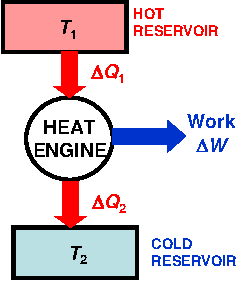
\includegraphics{"Statistical Physics and Entropy"/carnot_cycle}
	\end{center}
\end{figure}
The heat engine absorbs heat $\Delta Q_1$ from a hot reservoir at temperature $T_1$. But it cannot convert all of the heat $\Delta Q_1$ into work $\Delta W$. So, some heat must be rejected as $\Delta W$ waste heat $\Delta Q_2$ to a cold reservoir at temperature $T_2<T_1$. $\Delta U = 0$ and $\Delta S = 0$ for the engine in a complete cycle. Entropy of hot reservoir decreases by $\frac{\Delta Q_1}{T_1}$ and the entropy of cold reservoir increases by $\frac{\Delta Q_2}{T_2}$.

\subsubsection{Efficiency of the Carnot Cycle}
$\Delta U = 0$ and $\Delta S = 0$ for the engine in a complete cycle. The entropy of the hot reservoir decreases by $\frac{\Delta Q_1}{T_1}$. The entropy of cold reservoir increases by $\frac{\Delta Q_2}{T_2}$. 
\begin{align*}
		\text{First Law} &\qquad \Delta W = \Delta Q_1 - \Delta Q_2 \\
		\text{Second Law} &\qquad \Delta S_\text{total} = \frac{\Delta Q_2}{T_2} - \frac{\Delta Q_1}{T_1} \ge 0
\end{align*}
The efficiency is given by $\eta = \frac{(\text{Work Out})}{(\text{Heat In})}$
\[
	\Rightarrow \eta = \frac{\Delta W}{\Delta Q_1} \le \frac{(T_1 - T_2)}{T_1}
\]
The equality only applies to a reversible Carnot cycle.This implies that no heat engine can be more efficient than an ideal Carnot Engine, which executes a reversible Carnot cycle. The maximum efficiency is $\eta = \frac{(T_1 - T_2)}{T_1}$ (typically around 40\%). Waste heat is unavoidable (unless we let $T_2 \rightarrow 0$).
\begin{figure}[h]
	\begin{center}
		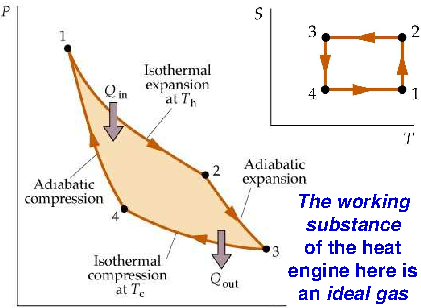
\includegraphics{"Statistical Physics and Entropy"/carnot_cycle_graph}
	\end{center}
\end{figure}

\subsubsection{The Rankine Section}
This is a similar cycle for steam engines.
\begin{figure}[h]
	\begin{center}
		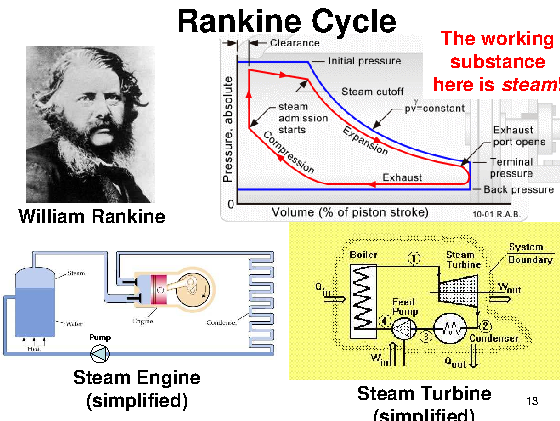
\includegraphics{"Statistical Physics and Entropy"/rankine_cycle}
	\end{center}
\end{figure}






\includepdf{\string"Statistical Physics and Entropy/\string"Syllabus} 
\end{document}
